\documentclass[12pt,a4paper]{article}

% 如果需要中文支持,推荐使用xeCJK + 字体设置
\usepackage{xeCJK}
\setCJKmainfont{SimSun}  % 示例:宋体,可根据系统字体情况更换
\usepackage{amsmath}      % 数学公式(如有需要)
\usepackage{graphicx}     % 插图
\usepackage{geometry}     % 调整页边距
\usepackage{fancyhdr}     % 自定义页眉页脚
\usepackage{indentfirst}  % 中文首行缩进
\usepackage{calc}         % 允许做长度运算(测量文字宽度等)
\usepackage{titlesec}
\usepackage{booktabs} % 解决 \midrule 和 \bottomrule 报错
\usepackage{enumitem} % 支持自定义列表格式
\usepackage{float}
\usepackage{subcaption}
\usepackage{tabularx}
\usepackage{float}

% 设置 \section 级标题为:加粗、大字号(如 \Large)
\titleformat{\section}
	{\bfseries\large}    % 标题自身的格式
	{\thesection}        % 标题编号的显示方式
	{1em}                % 编号与标题文字之间的间距
	{}                   % 在标题文字前后可插入额外代码,此处为空
	
% 设置 \subsection 级标题为:加粗、中等字号(如 \normalsize)
\titleformat{\subsection}
	{\bfseries\normalsize}
	{\thesubsection}
	{1em}
{}

% 页面设置(可根据需要微调)
\geometry{
	left=2cm,
	right=2cm,
	top=1cm,
	bottom=1.5cm
}

% 不需要过大的行距,使用较接近单倍行距的设置
\renewcommand{\baselinestretch}{1}

% 仅在页脚居中显示页码,页眉保持为空
\pagestyle{fancy}
\fancyhf{}  % 清空默认的页眉页脚
\fancyfoot[C]{\thepage}
\renewcommand{\headrulewidth}{0pt}
\renewcommand{\footrulewidth}{0pt}

% 首行缩进2字符(中文习惯)
\setlength{\parindent}{0pt}
\setlength{\leftskip}{2em}

\begin{document}
	%-------------------------------------------------------
	% 1 并排两个minipage:左标题、右校徽
	%   - 0.65\textwidth + 0.35\textwidth = \textwidth
	%   - 如果校徽过大或过小,可改宽度,如 0.25\textwidth、0.3\textwidth 等
	%   - 如果想让标题更大,可将 \Huge 改成 \huge 或 \LARGE
	%-------------------------------------------------------
	\noindent
	\hspace{-2em}
	\begin{minipage}[c]{0.65\textwidth}
		\raggedright
		{\fontsize{40pt}{60pt}\selectfont 物理实验报告}
	\end{minipage}
	\begin{minipage}[c]{0.35\textwidth}
		\raggedleft
		% 强制把校徽拉大到 0.35\textwidth 宽度 (高度自动匹配)
		% 若想指定高度,可用 "height=3cm" 等. 二选一即可.
		
\includegraphics[width=\linewidth, trim={20cm 20cm 20cm 20cm}, clip]{university_logo.png}
	\end{minipage}

	\vspace{-1em}
	

	%下方画两条分割线,并在两线之间写学号、姓名、日期、时间
	
	\hrule
	\vspace{0.4em}
	\noindent
	\begin{tabular}{l l l l}
    学号:\underline{114514} & 姓名:\underline{SUSTech} &
    日期:\underline{2025/05/06} & 时间:\underline{周二下午}
	\end{tabular}
	\vspace{-0em}
	\par
	\hrule

	

	%正文示例

	
	\section{实验名称:直线运动规律的研究}
	
	\section{实验目的}
		\begin{enumerate}[label=\arabic*.]
			\item 利用气压技术测定物体的“瞬时”速度,加速度以及当地的重力加速度。
			\item 利用气压技术研究一维碰撞的三种情况,验证动量守恒和动能守恒定律。
			\item 定量研究一维碰撞中的动量损失和动能损失。
		\end{enumerate}

	\section{实验仪器}
		气垫导轨实验仪器、电子计时器、滑块、天平

	\section{实验原理}
		\subsection{平均速度和瞬时速度的测量}
			作直线运动的物体在 $\Delta t$ 时间内的位移为 $\Delta s$, 则物体在 $\Delta t$ 时间内的平均速度为	$v = \frac{\Delta s}{\Delta t}$
			当 $\Delta t \to 0$ 时, 平均速度趋近于一个极限值, 即物体在该点的瞬时速度. 但实验上直接测量某点的瞬时速度是很困难的, 一般在一定误差范围内(小于5\%), 用极短的 $\Delta t$ 内的平均速度代替瞬时速度.

		\subsection{匀变速直线运动}
			在一个平斜面上,设有一小滑块在恒定力的作用下做匀加速直线运动。设小滑块初速度为 \( v_0 \)、加速度为 \( a \)、运动时间为 \( t \) 和位移为 \( s \),则运动学关系可描述为:
			\[v = v_0 + at,\quad s = v_0 t + \frac{1}{2}at^2 \quad \Rightarrow \quad v^2 = v_0^2 + 2as\]
			当小滑块从不同的位置开始滑动(对于起始时刻可视为 \( v_0 = 0 \)),在同一位置测量其速度时,若绘制 \( v^2 \) 与 \( s \) 的关系图,将得到一条直线,其斜率为 \( 2a \)。

		\subsection{重力加速度的测定}
			\( h \) 为斜块的高度,\( L \) 为斜面的长度,块沿斜面下滑的加速度为:
			\[a = g\sin\theta = g\frac{h}{L} \quad \Rightarrow \quad g = \frac{aL}{h}\]

		\subsection{碰撞过程中守恒定律的研究}
			如果一个力学系统所受合外力为零或在某方向上的合外力为零,则该力学系统总动量守恒或在某方向上守恒,即:$\sum m_i v_i = \text{constant}$
			对于三种碰撞情形,动量和动能守恒情形如下:
			\begin{itemize}
    			\item[(a)] 完全弹性碰撞:动量守恒,能量守恒
    			\item[(b)] 完全非弹性碰撞:动量守恒,动能不守恒
    			\item[(c)] 一般非弹性碰撞:动量守恒,动能不守恒
			\end{itemize}
	

	\section{实验内容}
		\subsection{匀变速运动中速度与加速度的测量}
			\begin{enumerate}
				\item 先将气囊导轨调平(动平调法:两光电门间距离50.00cm以上,轻轻推动大滑块,使其通过第一个光电门的时间 $t_1 > 80\,\text{ms}$,并且通过第二个光电门的时间 $t_2$ 满足 $t_1 - 5 < t_2 < t_1 + 5$),然后在一端单脚螺丝下置一滑块,使导轨成一斜面。
				\item 在大滑块上装上 U 型捆光片,调节光电门,打开展置,使用计形测试。
				\item 使大滑块分别从距离光电门 $S = 20.00\,\text{cm}, 30.00\,\text{cm}, 40.00\,\text{cm}, 50.00\,\text{cm}, 60.00\,\text{cm}$ 处自然下滑,进行初速度为零的匀加速运动,记下捆光时间 $\Delta t$,每个 $S$ 情况下重复测量三次。
				\item 测量 U 型捆光片有效长度 $\Delta s$(测3次)、斜面高度 $h$(测3次)及斜面长度 $L$(测1次)。
				\item 根据 U 型捆光片有效长度 $\Delta s$ 和捆光时间 $\Delta t$,计算出速度 $v$,用 Origin 软件进行直线拟合(提示:$v^2 = 2as$),求出加速度 $a$,并计算重力加速度 $g$(深检:$g \approx 9.7883\,\text{m/s}^2$)。
			\end{enumerate}
		\subsection{研究三种碰撞状态下的守恒定律}	
			\begin{enumerate}
				\item 撤掉气垫导轨的垫块,按计时器上的“功能”键,选择“碰撞”档位。
				\item 取大小两滑块A、B,将两滑块分别装上弹簧钢圈,用物理天平称此时滑块A、B的质量,分别记为 $m_1$ 和 $m_2$,且证明 $m_1 > m_2$。打开气泡,将小滑块B置于两光电门之间(两光电门的距离为30.00--40.00 cm),使其静止。用 $m_1$ 碰 $m_2$,分别记为 $m_1$ 通过第一个光电门的时间 $\Delta t_{11}$ 和经过第二个光电门的时间 $\Delta t_{12}$,以及 $m_2$ 通过第二个光电门的时间 $\Delta t_{21}$,重复三次,记录所测数据。
				\item 分别在两滑块上换上尼龙搭扣,重复上述测量步骤。
				\item 分别在两滑块上换上金属碰撞器,重复上述测量步骤。
				\item 分别计算每种碰撞下动量的变化、动能的变化,计算动量损失率 $\Delta p/p$ 和动能失率 $\Delta E/E$,并根据计算数据得出相应的实验结论。
			\end{enumerate}
		
	\section{数据记录}
	  根据实验原理及实验内容进行实验,并输入excel进行统计计算。

	\section{数据处理}
	  	\subsection{匀变速运动中速度与加速度的测量}
		  	\begin{figure}[H]
				\centering
				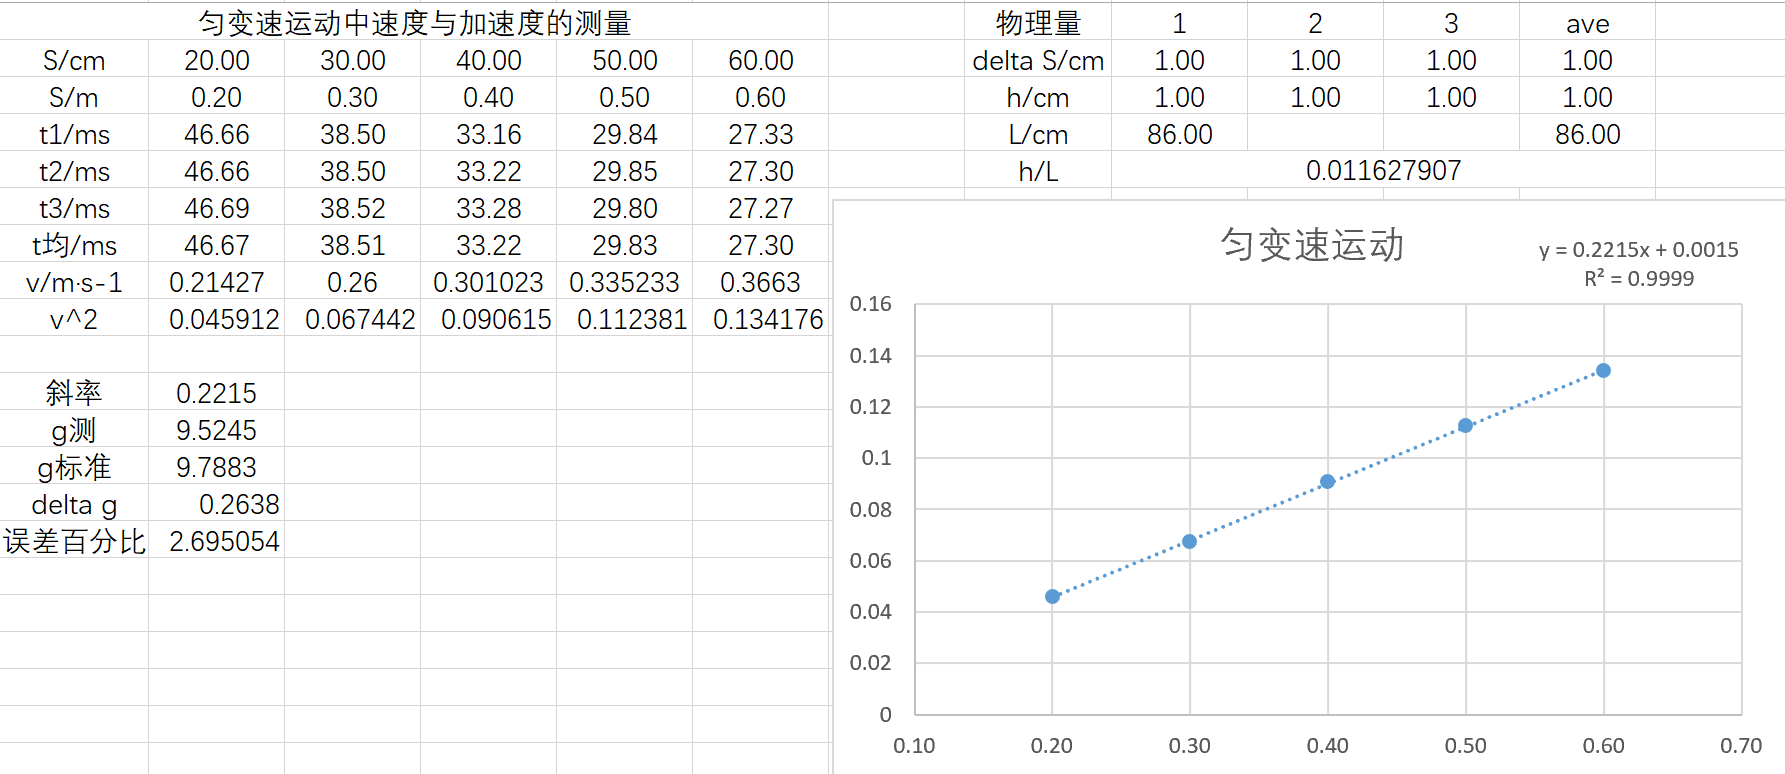
\includegraphics[width=0.75\textwidth]{图1.png}
				\caption{匀变速运动中速度与加速度的测量}
				\label{fig:数据}
	  		\end{figure}
			根据公式$v=\frac{\Delta s}{t}$可计算$v$及$v^2$,再作出$v^2—s$图,通过线性回归拟合得方程为$y=0.2215x+0.0015,R^2=0.9999$。由公式$g = \frac{aL}{h}$计算可得$g_{测}=9.5245\,\text{m/s}^2$;
			深圳地区的标准重力加速度为$g_{深圳}=9.7883\,\text{m/s}^2$
			因此,重力加速度的相对误差(百分比)为$\eta=\frac{\lvert g_{深圳}-g_{测} \rvert}{g_{深圳}}\times 100\% \approx 2.695\%$
			
	  	\subsection{研究三种碰撞状态下的守恒定律}

			\subsubsection{完全弹性碰撞}
				\begin{figure}[H]
					\centering
					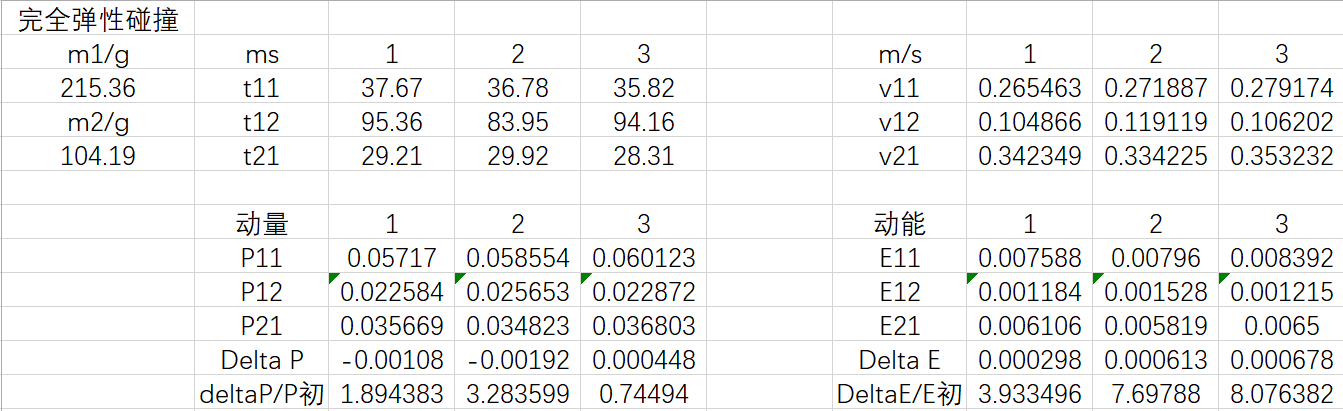
\includegraphics[width=0.75\textwidth]{完全弹性碰撞.png}
					\caption{完全弹性碰撞}
					\label{fig:数据}
	  			\end{figure}
				由公式$p=mv,E_k=\frac{1}{2} m v^2$可得,
				$$\eta_{p1}=\Delta p/p=1.89\%<5\%,\eta_{p2}=\Delta p/p=3.28\%<5\%,\eta_{p3}=\Delta p/p=0.75\%<5\%$$
				$$\eta_{E1}=\Delta p/p=3.93\%<5\%,\eta_{E2}=\Delta p/p=7.69\%>5\%,\eta_{E3}=\Delta p/p=8.08\%>5\%$$
				在误差与许范围内:动量守恒,能量守恒

			\subsubsection{完全非弹性碰撞}
				\begin{figure}[H]
					\centering
					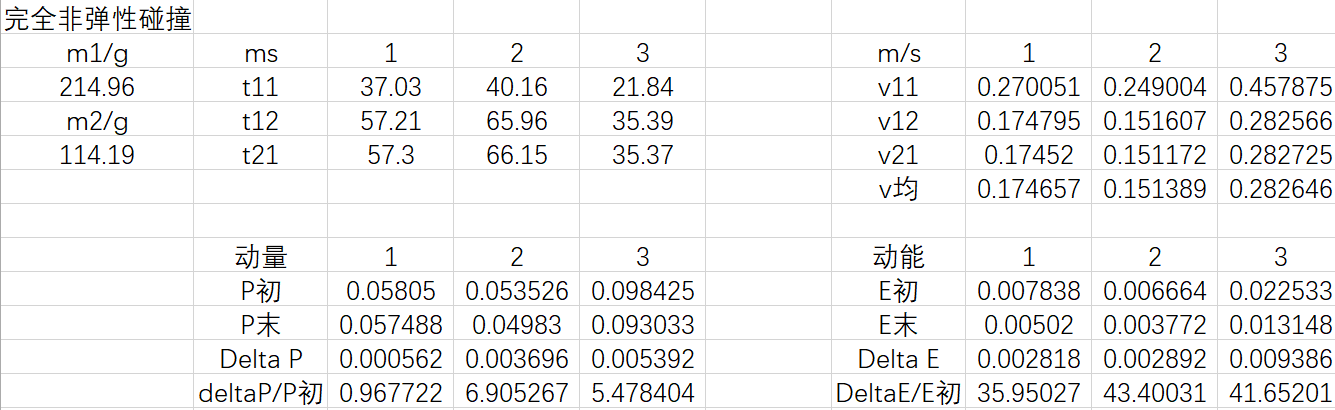
\includegraphics[width=0.75\textwidth]{完全非弹性碰撞.png}
					\caption{完全非弹性碰撞}
					\label{fig:数据}
	  			\end{figure}
				由公式$p=mv,E_k=\frac{1}{2} m v^2$可得,
				$$\eta_{p1}=\Delta p/p=0.97\%<5\%,\eta_{p2}=\Delta p/p=6.91\%>5\%,\eta_{p3}=\Delta p/p=5.48\%>5\%$$
				$$\eta_{E1}=\Delta p/p=35.95\%>5\%,\eta_{E2}=\Delta p/p=43.40\%>5\%,\eta_{E3}=\Delta p/p=41.65\%>5\%$$
				在误差与许范围内:动量守恒,动能不守恒

			\subsubsection{一般非弹性碰撞}
				\begin{figure}[H]
					\centering
					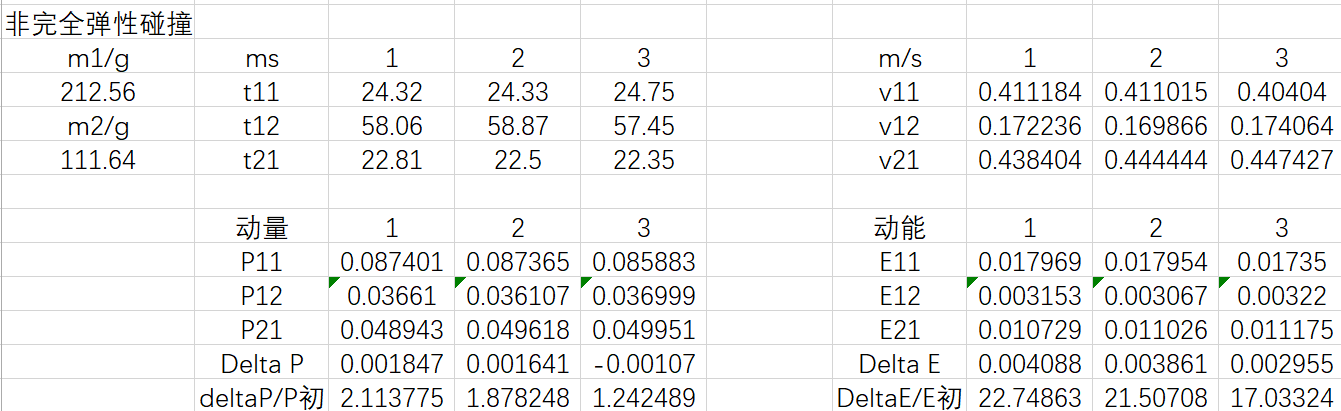
\includegraphics[width=0.75\textwidth]{一般非弹性碰撞.png}
					\caption{一般非弹性碰撞}
					\label{fig:数据}
	  			\end{figure}
				由公式$p=mv,E_k=\frac{1}{2} m v^2$可得,
				$$\eta_{p1}=\Delta p/p=2.11\%<5\%,\eta_{p2}=\Delta p/p=1.88\%<5\%,\eta_{p3}=\Delta p/p=1.24\%<5\%$$
				$$\eta_{E1}=\Delta p/p=22.75\%>5\%,\eta_{E2}=\Delta p/p=21.51\%>5\%,\eta_{E3}=\Delta p/p=17.03\%>5\%$$
				在误差与许范围内:动量守恒,动能不守恒

		\subsection{误差分析}
				\begin{itemize}
					\item 存在空气阻力等影响,不能认为完全无阻力
					\item 气垫导轨未完全调平
					\item 难以控制$\Delta t$在20——100ms区间
					\item 手动难以使滑块以绝对静止,从距光电门无误差位置下滑
				\end{itemize}
				
	\section{思考题}
		\begin{enumerate}
			\item 气垫导轨调水平的判断标准是什么?\\
			气垫导轨调水平的主要判断标准是观察放置其上的滑块是否能够保持静止或做匀速直线运动。若滑块在不同位置均能静止不滑动,或被轻推后能保持匀速运动,则表明导轨已基本水平。更精确地,可借助高精度气泡水平仪辅助调整。
		
			\item 如何减小气垫导轨气流阻力对实验的影响?\\
			减小气流阻力的主要方法包括:确保足够的气压和气流量以形成稳定的气垫;保持导轨和滑块表面的清洁光滑;优化滑块的形状以减小空气阻力;以及在实验操作上尽量缩短实验时间和滑块的运动距离。
		
			\item 碰撞前后系统总动量不相等(可能出现碰撞后动量减小或增加),试分析其原因。\\
			碰撞前后系统总动量不相等的主要原因在于实际实验中存在外力作用,如导轨不完全水平导致的重力分力、残余的摩擦力和空气阻力等。此外,测量误差以及系统并非完全封闭(如能量散失)也会导致动量看似不守恒。若出现动量增加,则可能存在系统内能转化为动能的过程。
		\end{enumerate}


	\section{实验结论}
	1. 测量重力加速度$g \approx 9.5245 \approx 9.62 \,\text{m/s}^2$,相对误差$\eta \approx 2.69\%$



2. 对于不同碰撞状态下:
\begin{itemize}
    \item 完全弹性碰撞:\\
		动量损失率为 $$\eta_{p1}=\Delta p/p=1.89\%<5\%,\eta_{p2}=\Delta p/p=3.28\%<5\%,\eta_{p3}=\Delta p/p=0.75\%<5\%$$
		动能损失率为 $$\eta_{E1}=\Delta p/p=3.93\%<5\%,\eta_{E2}=\Delta p/p=7.69\%>5\%,\eta_{E3}=\Delta p/p=8.08\%>5\%$$
		即:在误差与许范围内:动量守恒,能量守恒
    \item 非完全弹性碰撞:\\
		动量损失率为 $$\eta_{p1}=\Delta p/p=0.97\%<5\%,\eta_{p2}=\Delta p/p=6.91\%>5\%,\eta_{p3}=\Delta p/p=5.48\%>5\%$$
		动能损失率为 $$\eta_{E1}=\Delta p/p=35.95\%>5\%,\eta_{E2}=\Delta p/p=43.40\%>5\%,\eta_{E3}=\Delta p/p=41.65\%>5\%$$
		即:在误差与许范围内:动量守恒,能量不守恒
    \item 完全非弹性碰撞:\\
		动量损失率为 $$\eta_{p1}=\Delta p/p=2.11\%<5\%,\eta_{p2}=\Delta p/p=1.88\%<5\%,\eta_{p3}=\Delta p/p=1.24\%<5\%$$
		动能损失率为 $$\eta_{E1}=\Delta p/p=22.75\%>5\%,\eta_{E2}=\Delta p/p=21.51\%>5\%,\eta_{E3}=\Delta p/p=17.03\%>5\%$$
		即:在误差与许范围内:动量守恒,能量不守恒
\end{itemize}
	

\end{document}
